
\chapter{Discrete distributions}

\section{Random variables and sampling}
\subsection{Types of sampling}

\begin{enumerate}
    \item \textbf{Sampling with replacement}: Outcomes are independent.
    \item \textbf{Sampling without replacement}: Outcomes are dependent.
    \item \textbf{Sampling without replacement with small sample size compared to population}: Can assume that outcomes are pretty much independent.
\end{enumerate}

\qs{}{
    Suppose that in a very large city 20\% of people have a genetic mutation. If 10 people are examined, what is:
    \begin{enumerate}
        \item The probability that exactly two have the mutation?
        \item The probability that at least two will have the mutation?
    \end{enumerate}
}

\sol{
    We are sampling without replacement. Let the outcome on trial $i$ be:\\
    $M_i$: the i-th individual has the mutation.\\
    $M^ci$: the i-th individual does not haev the mutation..\\

    for $i = 1, 2, ...10$.\\

    Let $X = $ \# of mutations in these 10 trials.\\

    To find $P(X=2)$, we first find probability of a specific configuration of mutations and non-mutations in 10 trials that results in two mutations out of 10. We will sum up the probabilities of all such configurations.\\

    One such configuration is:
    $$M_1 \cap M_2 \cap M^c_3 \cap M^c_4 \cap ... \cap M^c_{10}$$
    $$=P(M_1 \cap M_2 \cap M^c_3 \cap M^c_4 \cap ... \cap M^c_{10})$$
    $$=P(M_1) P(M_2) P(M^c_3) ... P(M^c_{10})$$ (by independence - one person having a mutation does not influence another person having the mutation)
    $$=(0.2)^2 (0.8)^2$$

    We can read this as there being a 20\% chance that one person having the mutation. In reality if we are sampling without replacement, there would be a slightly higher chance that the next person picked has the mutation. With a very large population this effect is negligible. So we assume independence of events.\\

    Every configuration includes 2 people with the mutation ($(0.2)^2$ chance) and 8 people without the mutation ($(0.8)^2$ chance).\\

    The number of possible configurations of 2 people with mutations is given by $\binom {10}{2}$ (number of ways to pick 2 mutations from 10, where order does not matter). Each configuration with 2 mutations has a probability $(0.2)^2(0.8)^2$ of occurring. Each configuration is disjoint.\\

    Therefore, the total probability of any of these configurations occurring is $\binom {10}{2} (0.2)^2(0.8)^8$.\\

    General formula:

    $$P(X \ge 2) = \sum_{k=2}^{10} (P(X = k))$$
    $$P(X \ge 2) = \sum_{k=2}^{10} (0.2)^{k} (0.8)^{10-k} \binom {10}{k}$$

    Or, by using the complement:

    $$P(X \ge 2) = 1 - P(X < 2)$$
    $$P(X \ge 2) = 1- \{ P(X=0) + P(X = 1) \}$$
    $$P(X \ge 2) = 1 - (0.2)^2(0.8)^1 0 \binom{10}{0} - (0.2)^2(0.8)^9 \binom{10}{1}$$
    
}

\dfn{Random variable}{
    A random value is a real-valued function defined over a sample space.
}

\ex{}{
    Toss 3 fair coins. Let $X = $ \# of tails observed. Then $X = 0, 1, 2, 3$. Each has an associated probability: $P(X = x)$.
}

\begin{figure}[H]
    \centering
    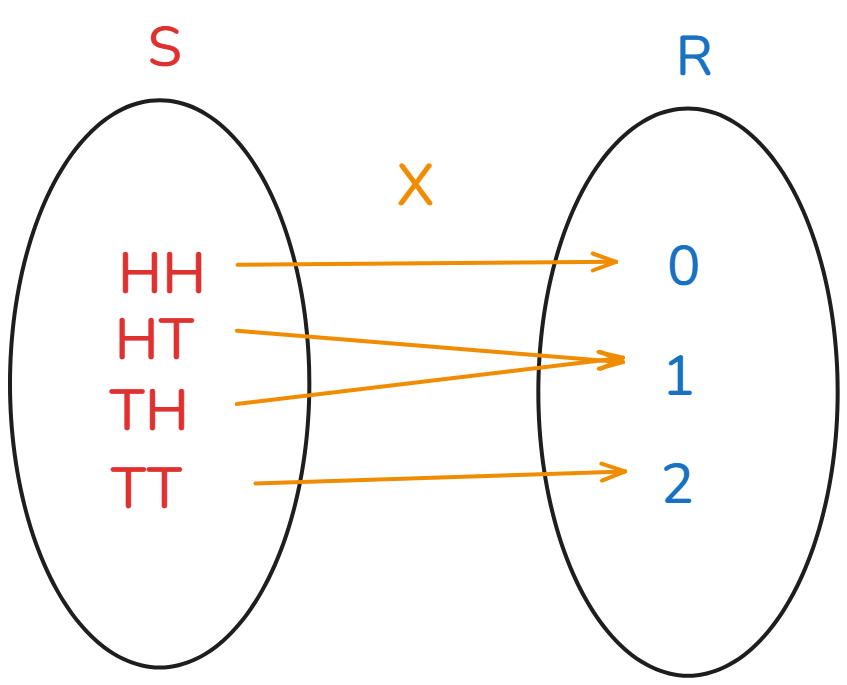
\includegraphics[width=0.5\linewidth]{images/random_var.png}
    \caption{Random variable function}
\end{figure}

\subsection{Discrete random variable distribution}
\dfn{Discrete random variable}{
    A random variable is \textbf{discrete} if its range is finite or countably infinite. Then the set of values that $X$ can take can be described as: $R_x = \{ x_1, x_2, ... \}$.
}

\dfn{Probability distribution}{
    Probability distribution can be described as $\rho(x) = P(X = x) \forall{x}$. Then $\sum_{x=0}^{n} P(X = x) = 1$
}

\dfn{Cumulative distribution function} {
    Defined as: 
    $$F_X (x) = P(X \le x), \forall{x} \in R$$

    The domain of $F_X (x)$ is the real line. The range is $[0,1]$.
}

\begin{figure}[H]
    \centering
    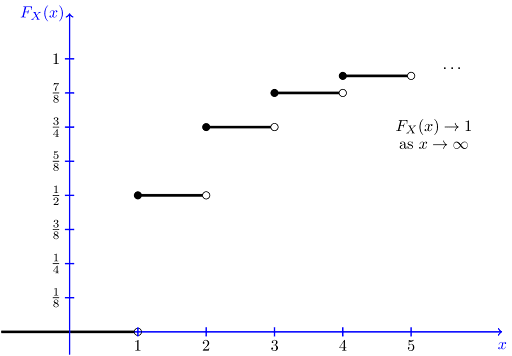
\includegraphics[width=0.6\linewidth]{images/cum_dist.png}
    \caption{Cumulative distribution function}
    \label{fig:enter-label}
\end{figure}

\ex{}{
    Recall the 3 coin throws.

    $$P(X \le 1) = P(X = 0) + P(X = 1)$$

    $$F_X (1) = P(X \le 1)$$
}

\nt{
    Possible to write individual probabilities as difference of cumulative probabilities. For example:

    $$F_X(2) - F_X(1) = P(X = 2)$$

    More generally:

    $$P(X=x_k) = F_X (x_k) - F_X (x_k - \epsilon)$$
}

\pagebreak

\textbf{Properties of CDF}\\

\begin{enumerate}
    \item $x \le y$, then $F_X (x) \le F_X (y)$
    \item $lim_{x\rightarrow + \inf} F_X (x) = 1$
    \item $lim_{x\rightarrow - \inf} F_X (x) = 0$
    \item Right continuous
\end{enumerate}

\nt{ 
    Mathematical expression for right continuity is:
    
    $$lim_{x \rightarrow x^+_k} F_X (x) = F_X (x_k)$$
    
    for $x_k \le x < x_{k+1}$
}


\dfn{Probability mass function}{
    The probability mass function of a discrete random variable is give by:

    $$P_X(x_k) = P(X=x_k)$$

    Where $P_X(x_k) = P(X = x_k) > 0$ if $x_k \in R_X$ and $P_X(x_k) = 0$ if $x_k \not \in R_X$
}

\dfn{Discrete uniform distribution}{
    A random variable $X$ is said to have a discrete uniform distribution if for $x_1, x_2, ... x_n \in R$ where $R$ is the set of real numbers:

    $$\rho_X (x) = P(X = x) = \frac{1}{N}$$

    for $X = x_1, x_2, ... x_N$

}

\begin{figure}[H]
    \centering
    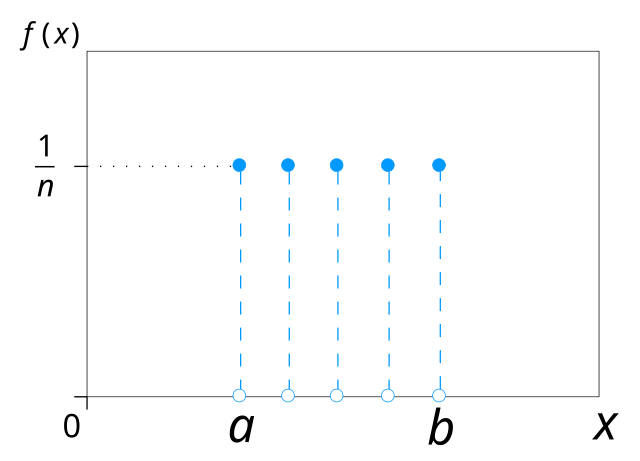
\includegraphics[width=0.5\linewidth]{images/uniform_dist.png}
    \caption{Discrete uniform distribution}
    \label{fig:enter-label}
\end{figure}

\ex{}{
    Throw a fair die. The possible outcomes are $\{1, 2, 3, 4, 5, 6\}$. The random variable $X$ takes the values $X = 1, 2, 3, 4, 5, 6$.

    $$P(X = x_i) = \frac{1}{6}$$

    for all $x_i \in \{1, 2, 3, 4, 5, 6\}$

}

\dfn{Bernoulli Distribution}{
    A random $X$ is said to have a Bernoulli Distirbution if $X$ can take only two possible values, usually $0$ and $1$. Is used to model situation where random experiment that has two possible outcomes, usually referred to as "success" or "failure".\\

    Probability of success is denoted $p$, $0 < p < 1$.\\

    Then probabilty distribution is given by:

    \begin{equation}
        P(X = x)
        \begin{cases}
            p^x(1-p)^{1-x} \text { if } x \in \{0, 1\}\\
            0 \text{ otherwise }
        \end{cases}
    \end{equation}
}

\section{Binomial distribution}

\dfn{Binomial experiment}{
    An experiment is called a binomial experiment if it consists of $n$ independent Bernoulli trials (trial with two outomes: success and failure). The probability of success $p$ remains constant from trial to trial. We are interested in $x$ successes out of $n$ trials. 
}

\dfn{Binomial distribution}{
    Let $X$ be the random variable that counts the number of successes in $n$ \textbf{independent} Bernoulli trials, where the probability of success remains \textbf{constant} from trial to trial. The probability distribution is denoted:
    $$X \sim \text{Binom}(n,p)$$
}

\ex{}{
    According to tables by the National Centre for Health Sciences
    in Vital Statistics for United States, a person at the age of 20 years has a probability of 0.8 of being alive at the age of 65 years. Suppose three people of age 20 years are chosen at random (all people in the population of 20 years old the US are equally likely to be chosen).

    Let $A_i$ be the event that the $i^{th}$ person chosen will be alive at the age of 65. Then $A_i^c$ is the event that the $i^{th}$ person chosen will not be alive at the age of 65.

    We are given that a person at the age of 20 years has the probability of 0.8 at the age of 65 years.

    Two possible outcomes: alive or dead, so these are Bernoulli trails. Then the random experiment of observing whether a person is alive at the age of 65 can be modelled by using Bernoulli random variable. 

    Let $X$ be the random variable that takes values 0 or 1 where 0 corresponds to not alive and 1 corresponds to being alive at the age of 65.

    Number of possible ways you can observe a given event is the number of ways it occurs $\binom {n}{x}$ times the probability tha it occurs. For example, in a sample of $3$, to observe if $2$ are alive at age of 65, you would find this by $\binom{3}{2} (0.8)^2(0.2)^1 = 0.384$. 
}

\thm{Binomial distribution}{
    For a binomial random variable $X$

    $$P(X=x) = \binom{n}{x} p^{x} (1-p)^{n-x}$$

    where $x = 0, 1, ... n$

}

\qs{}{
    Suppose that a lot of 5000 electrical fuses contains 5\% defectives. If a sample of 5 fuses is tested, find the probability of observing at least one defective.
}

\sol{
    There are two outcomes: defective or not defective. Can represent $X$ (number of successes) in $n$ trials as a binomial random variable.
    $$n = 5$$
    $$X \sim \text{Binom}(5,0.5$$
    Then to find at least one defective:
    $$P(X \ge 1) = P(X=1) + P(X=2) + P(X = 3) + P(X=4) + P(X = 5)$$
    $$= \sum_{x=1}^{5} \binom {5}{x} (0.05^x)(0.95)^{5-x}$$
    $$P(X \ge 1) = 1 - P(X = 0)$$
    $$= 1 - \binom{5}{0} (0.05)^0 (0.95)^5$$
}

\section{Geometric distribution}

\dfn{Geometric distribution}{
    A random variable $X$ is said to have geometric distribution if the sample space countains a \textbf{countably infinite} number of sample points, where we are looking for the probability that an event first occurs on the $x^{th}$ trial.
}

\thm{}{
    Let $X$ be the trial at which the first success occurs. Then
    $$P(X = x) = (1-p)^{x-1}p$$
    $$0 < p < 1, x = 1, 2, 3, ...$$
}

\pf{Proof}{
    The event $X = x$ can be expressed as :

    $$\{ X = x \} = \{ FFFF ... F S \}$$ 
    
    where we observe $x - 1$ failures. Let $p$ be the probability of success.

    $P(X = x) = P(F \cap F \cap F ... \cap F \cap S)$
    $$= P(F) ^{x-1} P(S)$$
    $$= (1-p)^{x-1} p$$
}

\qs{}{
    You ask people outside a polling station who they voted for until you find someone that voted for the Liberal candidate in a recent election. The probability that a randomly chosen person votes a liberal candidate is 0.4 What is the probability that the first person who voted for the Liberals is the fifth person you interviewed?
}

\sol{
    Using geometric distribution. We are finding $X = 5$ and $p = 0.4$:

    $$P(X = 5) = (1-0.4)^{4} (0.4)$$
    $$P(X = 5) = 0.05184$$
}

\section{Negative binomial distribution}
\dfn{Negative binomial distribution}{
    Let $X$ be a negative binomial random variable. Then:
    $$P(X=x) = \binom{x-1}{r-1} p^r (1-p)^{x-r}$$
    where $x = r, r+1, ...$. We write this as $X \sim NB(r, p)$ where $r$ is the number of successes. Then this is the probability of getting the $r$-th success on the $x$-th trial.
}

\pf{Proof}{
    The event $\{ X = x \}$ can be written as:
    $$\{ X = x \} = \{ r - 1 \text{ successes in x - 1 trials } \} \cap \{ \text{r-th success on xth trial} \}$$
    $$P(X = x) = P(E_1 \cap E_2)$$
    $$= P(E_1) \cdot P(E_2)$$
    $$=\binom{x-1}{r-1}p^{r-1} (1-p)^{(x-1)-(r-1)} \cdot p$$
    $$=\binom{x-1}{r-1} p^r (1-p)^{x-r}$$
    
}

\qs{}{
    An oil company conducts a geological study that indicates that an exploratory oil well should have a 20\% chance of striking oil. What is the probability that the third strike comes on the seventh well drilled?
}


\sol{}{
    $$ x = 7$$
    $$x \sim NB(3, 0.2)$$

    $$P(x = 7) = \binom{6}{2} (0.3)^3 (0.8)^4$$
}

\section{Poisson distribution}
\dfn{Poisson distribution}{
    Let $x$ be the number of successes in a unit time interval or unit space. let $\lambda$ be the average number of events that occur within a given interval of time or space.

    $$P(X=x) = \frac{ \lambda ^x e^{-\lambda}}{x!}$$
    $$x = 0, 1, 2, ...$$
}

\ex{}{
    Show that the probabilities assigned by the Poisson probability distribution satisfy that $\sum_{X=0}^{\infty} p(x) = 1$ for all $x$.
}

\sol{}{
    $$\sum_{x=0}^{\infty} \frac{\lambda ^x e^{-\lambda}}{x!}$$
    $$= e^{-\lambda} \sum_{x=0}^{\infty} \frac{\lambda ^2}{x!}$$
    We recognize this as a Maclaurin series for $e^\lambda$.
    $$= e^{-\lambda} ( \frac{\lambda ^ 0}{0!} + \frac{\lambda ^ 1}{1!}  + ... )$$
    $$= e^{-\lambda} \cdot e^{\lambda}$$
    $$= 1$$
}

\thm{}{
    Let $X \sim Binom(n,p)$. Then for $np = \lambda$, we have:

    $$lim_{n \to \infty} P(X = x) = \frac{ \lambda ^x e^{-\lambda}}{x!}$$
    $$lim_{p \to 0} P(X = x) = \frac{ \lambda ^x e^{-\lambda}}{x!}$$

    In other words, the bimomial distribution is approximated by the Poisson approximation when $n \rightarrow \infty$ and $p \rightarrow 0$.
}

\pf{Proof}{
    Let $X \sim Binom(n,p)$, where $n \rightarrow \infty$ and $p \rightarrow 0$ and $np = \lambda$. Then:
    $$lim_{n \to \infty} P(X = x) = \lim_{n \to \infty} \binom{n}{x} p^x (1-p)^{n-x}$$
    $$= \lim_{n \to \infty} \binom{n}{x} (\frac{\lambda}{n})^x (1- \frac{\lambda}{n})^{n-x}$$
    $$=\lim_{n \to \infty} \frac{n!}{(n-x)! x!} \frac{\lambda ^2}{n^2} (1 - \frac{\lambda}{n})^n \cdot (1 - \frac{\lambda}{n})^{-x}$$
    $$=\frac{\lambda^x}{x!} (\lim_{n \to \infty} \frac{1}{n^x} \frac{n!}{(n-x)!} (1-\frac{\lambda}{n})^n )(1-\frac{\lambda}{n})^{-x} )$$
    We consider each of the factors separately. Considering only $$\lim_{n \to \infty} \frac{1}{n^x}\frac{n!}{(n-x)!}$$
    $$=\lim_{n \to \infty} \frac{n(n-1)(n-2)... (N-(x-1))}{n^x}$$
    $$\lim_{n \to \infty} 1 \cdot (1 - \frac{1}{n}) (1- \frac{2}{n}) ... (1 - \frac{x-1}{n})$$
    Recall that:
    $$lim_{n \to \infty} (1 + \frac{1}{n})^n = e$$
    $$lim_{n \to \infty} (1 - \frac{\lambda}{n})^n = e^{-\lambda}$$

    This means that
    $$lim_{n \to \infty} (1 - \frac{\lambda}{n})^n = e^{-\lambda}$$

    Finally, consider 
    $$lim_{n \to \infty} (1 - \frac{\lambda}{n})^{-x}$$
    $$= \lim_{n \to \infty} \frac{1}{(1 - \frac{\lambda}{n})^x}$$

    Therefore, multiply all these limits (taken separately) together:

    $$lim_{n\infty} P(X = x) = \frac{\lambda ^x}{x!} e^{-\infty}$$

}

\nt{
    When the value of $n$ in a binomial distribution is large and the value of $p$ is very small, binomial distribution can be approximated by a Poisson distribution. If $n \ge 100$ and $np \le 10$ then the Poisson distribution provides a good approximation to the binomial distribution.
}

\qs{}{
    Suppose that sections of textile length 1cm have a flaw in them with probability 0.01. If 1000 such sections are examined, what is the probability that:\\
    a. exactly 10 will have a flaw?
    b. at least 50 will have a flaw?
}

\sol{}{
    a. Looking for $P(X = 10)$. We can model this using a binomial distribution: $x \sim Binom(1000, 0.01)$. Then:
    $$P(X = 10) = \binom{n}{x}p^{x} (1-p)^{n-x} $$
    $$= \binom{1000}{10}(0.01)^{10} (0.9)^{990}$$
    But because $n$ is large and $np$ is small, we can approximate the binomial distribution by the Poisson distribution.
    $$P(X = 10) = \frac{\lambda ^x e^{-\lambda}}{x!}$$
    $$ = \frac{10^{10} e^{-10}}{10!}$$
}

\qs{}{ 
    Industrial accidents occur according to a Poisson process with an average of 3 accidents pers month. What is the probbaility of 10 accidents during the last 2 months?
}

\sol{}{
    The number of accidents in two months, $X$ has Poisson probability distribution with mean $\lambda ^{t} = 2(3) = 6$.
}

\section{Hypergeometric distribution}
\dfn{}{
    Let $N$ be the sample size. Let $a$ be the number of favorable items in total sample space. Let $x$ be the number of favorable items in a sample of size $n$. Then:
    $$P(X = x) = \frac{\binom{a}{x}\binom{N-a}{n-x}}{\binom{N}{n}}$$
    Write as $X \sim hypergeometric(N, n, a)$ where $x = 0, 1, 2, ... min(a,n)$. 
}


\section{Expectation and variance}

The expected value of a random variable $X$ is the measure of centrality of $X$. It is the weighted mean or average of all possible values of the random variable $X$.

\dfn{}{
    Let $X$ be a discrete random variable with the possible values $\{ x_1, x_2, x_3, ... \}$ (finite or countably infinite). The expected value of $X$, denoted $E(X)$, is defined as:
    $$E(X) = \sum x_k P(X = x_k)$$
}

\ex{}{
    Rolling a fair die. The expected value is given by:

    $$E(X) = \frac{1}{6}(1 + 2 + 3 + 4 + 5 + 6)$$
    $$E(X) = 3.5$$
}


\textbf{Properties of expected variable}
\begin{enumerate}
    \item The expected value of X can be thought of as a long run average of X.
    \item The expected value of X exists if E|X| converges.
\end{enumerate}

\qs{}{ 
    Consider the probability mass function $P(X = x) = \frac{c}{x^2}$ of the random variable $X$, where $x = 1, 2, ...$. Find the expected value of $X$.
}

\sol{}{
    $$E(x) = \sum_{x=1}^{\infty} x P(X = x)$$
    $$E(x) = \sum_{x=1}^{\infty} x \cdot \frac{x}{x^2}$$
    $$E(x) = \sum_{i=1}^{\infty} \frac{c}{x}$$
    $$E(x) = c \sum_{i=1}^{\infty} \frac{1}{x}$$

    This is a divergent series, so the expected value of $x$ does not exist.
}


\dfn{Mathematical expectation}{
    When it exists, the mathematical expectation satisfies the following properties. if $a$ is a constant, then:
    \begin{enumerate}
        \item $E(a) = a$
        \item If $a$ is a constant, then $E(aX) = aE(X)$.
        \item The mathematical expectation is linear. That is:
        $$E(X_1 + X_2 + ... + X_n) = E(X_1) + E(X_2) + ... E(X_n)$$
        for any set of random variables $X_1, x_2, ... X_n$.
    \end{enumerate}
    Mathematical expectation follows properties of linear transformations. Let $a_1, a_2$ be two constants that when the mathematical expectation exists, satisfies the following property:
    $$E(a_1 X_1 + a_2 X_2) = a_1 E(X_1) + a_2 E(X_2)$$   
}

\qs{}{
    An insurance company issues a one-year \$1000 policy insuring against the occurrence A that historically happens to 2 out of every 100 owners of the policy. Administrative fees are \$15 per policy and are not part of the company's profit. How much should the company charge for the policy if it requires that the expected profit per policy be \$50?
}

\sol{}{
Let $C$ be premium for policy. Company's profit is $C - 15$ if event $A$ does not occur and $C - 15 - 1000$ if A does occur. Let $X$ be a random variable that represents the company's profit:
$$E(X) = 50 = (C-15)(0.98) + (C-15-1000)(0.02)$$
$$C = 85$$
}

\dfn{Variance}{
    The variance of a random variable $X$ with mean $E(X) = \mu_X$ is defined as:

    $$Var(X) = E[(X - \mu_X)^2]$$
    $$ = E[(X - E(X))^2]$$
}

\textbf{Properties of variance}
\begin{enumerate}
    \item The variance of the random variable $X$ is denoted by $$Var(X) = \sigma_X ^2$$
    \item The variance of a random variable $X$ is the expected value of $(X - \mu _X)^2$.
    \item $Var(cX) = c^2 Var(X)$
\end{enumerate}

\thm{}{
    $$Var(X) = E[X^2] - [E(X)]^2$$
}

\pf{Proof}{
    $$Var(X) = E[(X - \mu_x)^2]$$
    $$=E[X^2 - 2 \mu_X X + \mu_X ^2]$$
    $$=E[X^2] - 2E[\mu_X X] + E[\mu_X  ^2 ]$$
    $$=E[X^2] - 2E[X]E[X] + [E(X)]^2$$
    $$E[X^2] - [E(X)]^2$$
}

\qs{}{
    What is the variance of a fair dice throw?
}

\sol{}{
    Know that $E(X) = 3.5$. Then:
    $$\sigma_2 = Var(X) = E[X^2] - [E(X)]^2$$
    $$= \frac{91}{6} - [\frac{7}{2}]^2$$
    $$= 2.92$$

    $$\sigma_X = \sqrt{2.921} = 1.71$$
}

\subsection{Moments of a distribution}
\dfn{}{
    Let $X$ be a discrete random variable. Then the moments of $X$ around the origin are $E(X), E(X^2), ... E(X^k)$, where $E(X^r) < \infty$ for $r = 1 ,2, ... k$.
}

The mean of the random variable $E(X)$ is the first moment of $X$. The variance of the random variable $E(X - \mu)^2$ is the second moment of $X$ about the mean.

Solving system of linear equations, can obtain the mean and variance from the classical and factorial moments.

$$E[X] - E[X]$$
$$E[X^2] = E[X(X-1)] + E[X]$$

\dfn{}{
    Let $X$ be a random variable. Then the $r^{th}$ factorial moment of $X$ is:
    $$E(X_r) = E[X(X-1)... (X - (r-1))]$$
    $E(X)$: First factorial moment of $X$.\\
    $E[X(X-1)]$: Second factorial moment of $X$.
}

\subsection{Mean and variance of uniform distribution}
\dfn{}{
    A random variable $X$ is said to have a discrete uniform distirbution if $\rho_X (x) = P(X = x) = \frac{1}{N}$ for $X = x_1, x_2, ... x_N$. 
}

Mean:
    $$E(X) = \sum_{k=1}^{N} x_k P(X = x_k)$$
    $$=\sum_{k=1}^{N} x_k \rho_X (x)$$
    $$=\frac{1}{N} \sum_{k=1}^{N} x_k$$
    $$=\overline{x}$$

Variance:
$$E(X^2) = \sum_{k=1}^{N} x_k ^2 P(X = x_k)$$
$$= \sum_{k=1}^{N} x_k ^2 \rho_X (x)$$
$$= \frac{1}{N} \sum_{k=1}^{N} x_k ^2$$
$$Var(X) = E[X^2] - [E(X)]^2$$
$$=\frac{1}{N} \sum_{k=1}^{N} x_k ^2 - \overline{x}^2$$

\subsection{Mean and variance of Bernoulli distribution}

Recall the probability distribution of the Bernoulli random variable $X$:

\begin{table}[H]
\centering
\caption{Probability distribution of Bernoulli distribution}
\begin{tabular}{|c|c|}
\hline
x & P(X=x)\\
\hline
0 & 1-p\\
1 & p\\
\hline
\end{tabular}
\end{table}

Mean:
$$E(X) = 0(1-p)+1(p) = p$$
$$E(X^2) = 0^2(1-p) + 1^2(p) = p$$
$$Var(X) = E[X^2] - [E(X)]^2$$
$$=p-p^2 = p(1-p)$$

\subsection{Summary}
\begin{table}[H]
\centering
\caption{Mean and Variance of Probability Distributions}
\begin{tabular}{|c|c|c|c|c|c|}
\hline
Distribution & Support & Parameters & $P(X = x)$ & Mean & Variance \\
\hline
Uniform (Discrete) & $\{a, a+1, \dots, b\}$ & $a, b$ & $\frac{1}{b-a+1}$ & $\frac{a+b}{2}$ & $\frac{(b-a+1)^2 - 1}{12}$ \\
Bernoulli & $\{0, 1\}$ & $p$ & $p^x (1-p)^{1-x}$ & $p$ & $p(1-p)$ \\
Binomial & $\{0, 1, \dots, n\}$ & $n, p$ & $\binom{n}{x} p^x (1-p)^{n-x}$ & $np$ & $np(1-p)$ \\
Poisson & $\{0, 1, 2, \dots\}$ & $\lambda$ & $\frac{e^{-\lambda} \lambda^x}{x!}$ & $\lambda$ & $\lambda$ \\
Geometric & $\{1, 2, 3, \dots\}$ & $p$ & $(1-p)^{x-1} p$ & $\frac{1}{p}$ & $\frac{1-p}{p^2}$ \\
Negative Binomial & $\{r, r+1, \dots\}$ & $r, p$ & $\binom{x-1}{r-1} (1-p)^{x-r} p^r$ & $\frac{r}{p}$ & $\frac{r(1-p)}{p^2}$ \\
\hline
\end{tabular}
\end{table}